\let\negmedspace\undefined
\let\negthickspace\undefined
\documentclass[journal]{IEEEtran}
\usepackage[a5paper, margin=10mm, onecolumn]{geometry}
%\usepackage{lmodern} % Ensure lmodern is loaded for pdflatex
\usepackage{tfrupee} % Include tfrupee package

\setlength{\headheight}{1cm} % Set the height of the header box
\setlength{\headsep}{0mm}     % Set the distance between the header box and the top of the text
\usepackage{multicol}
\usepackage{gvv-book}
\usepackage{gvv}
\usepackage{cite}
\usepackage{amsmath,amssymb,amsfonts,amsthm}
\usepackage{algorithmic}
\usepackage{graphicx}
\usepackage{textcomp}
\usepackage{xcolor}
\usepackage{txfonts}
\usepackage{listings}
\usepackage{enumitem}
\usepackage{mathtools}
\usepackage{gensymb}
\usepackage{comment}
\usepackage[breaklinks=true]{hyperref}
\usepackage{tkz-euclide} 
\usepackage{pgfplots}
\pgfplotsset{compat=1.18}
\usepackage{listings}
% \usepackage{gvv}                                        
\def\inputGnumericTable{}                                 
\usepackage[latin1]{inputenc}                                
\usepackage{color}                                            
\usepackage{array}                                            
\usepackage{longtable}                                       
\usepackage{calc}                                             
\usepackage{multirow}                                         
\usepackage{hhline}                                           
\usepackage{ifthen}                                           
\usepackage{lscape}
\usepackage{tikz}
% Marks the beginning of the document
\begin{document}
\bibliographystyle{IEEEtran}
\vspace{3cm}

\title{Finding maximum value\\NCERT-10.4.3.1.4}
\author{EE24BTECH11056 - S.Kavya Anvitha}
\maketitle
%\newpage
\bigskip

\renewcommand{\thefigure}{\theenumi}
\renewcommand{\thetable}{\theenumi}
\textbf{Question:}\\
Find the roots of the quadratic equation 
\begin{align*}
    2x^2 + x + 4
\end{align*}
\section{\textbf{Matrix Method}}
We can solve it with the help of companion matrix.

If the given polynomial is,
\begin{align}
	P(x) = c_0 + c_1\,x + c_2\,x^2 + \dots + c_{n-1}\,x^{n-1} + x^n
\end{align}

Then the companion matrix is given as,

\begin{align}
	A = \myvec{0 & 0 & \dots & 0 & -c_0\\1 & 0 & \dots & 0 & -c_1\\0 & 1 & \dots & 0 & -c_2\\\vdots & \vdots & \vdots & \vdots &\vdots \\0 & 0 & \dots & 1 & -c_{n-1}}
\end{align}
For our equation,
\begin{align}
  P(x) =  2x^2 + x + 4
\end{align}
The companion matrix is given as,
\begin{align}
   A = \myvec{0 & -2\\1 & \frac{-1}{2}} 
\end{align}
We can find the eigenvalues using QR algorithm.

\begin{align}
   A_n = Q_n\,R_n\\
   A_{n+1} = R_n\,Q_n
\end{align}
The goal is to find the eigenvalues of this matrix using the QR algorithm.

\section*{Step 1: Compute the Initial QR Decomposition}
Start with the matrix:

\[
A = \begin{bmatrix}
0 & -2 \\
1 & -\frac{1}{2}
\end{bmatrix}
\]

\subsection*{Step 1a: Compute $Q$ using Gram-Schmidt Process}
The columns of $A$ are:

\[
\mathbf{a_1} = \begin{bmatrix}
0 \\
1
\end{bmatrix}, \quad
\mathbf{a_2} = \begin{bmatrix}
-2 \\
-\frac{1}{2}
\end{bmatrix}
\]

Normalize the first column:

\[
q_1 = \frac{\mathbf{a_1}}{\|\mathbf{a_1}\|} = 
\begin{bmatrix}
0 \\
1
\end{bmatrix}
\]

Compute the orthogonal vector for the second column:

\[
\mathbf{u_2} = \mathbf{a_2} - (q_1^\top \mathbf{a_2})q_1
\]

\[
= \begin{bmatrix}
-2 \\
-\frac{1}{2}
\end{bmatrix}
- \left( -\frac{1}{2} \right) \begin{bmatrix}
0 \\
1
\end{bmatrix}
= \begin{bmatrix}
-2 \\
0
\end{bmatrix}
\]

Normalize the second column:

\[
q_2 = \frac{\mathbf{u_2}}{\|\mathbf{u_2}\|} = 
\begin{bmatrix}
-1 \\
0
\end{bmatrix}
\]

Thus, the matrix $Q$ becomes:

\[
Q = \begin{bmatrix}
0 & -1 \\
1 & 0
\end{bmatrix}
\]

\subsection*{Step 1b: Compute $R$}
The matrix $R$ is given by:

\[
R = Q^\top A = \begin{bmatrix}
0 & 1 \\
-1 & 0
\end{bmatrix}
\begin{bmatrix}
0 & -2 \\
1 & -\frac{1}{2}
\end{bmatrix}
=
\begin{bmatrix}
-1 & 0 \\
1 & -2
\end{bmatrix}
\]

\subsection*{Step 1c: Compute the Next Iteration Matrix $C_1$}
\[
A_1 = RQ = \begin{bmatrix}
-1 & 0 \\
1 & -2
\end{bmatrix}
\begin{bmatrix}
0 & -1 \\
1 & 0
\end{bmatrix}
=
\begin{bmatrix}
0 & 1 \\
-2 & 0
\end{bmatrix}
\]

\section*{Step 2: Repeat the QR Iteration}
The QR steps will be repeated iteratively until the matrix converges to a quasi-upper triangular form.
\begin{align}
   A_n = Q_n\,R_n\\
   A_{n+1} = R_n\,Q_n
\end{align}
\section*{Step 3: Final Quasi-Upper Triangular Form}
Since the eigenvalues are complex, the matrix will converge to a block diagonal form:

\[
A_{\text{final}} \approx \begin{bmatrix}
-\frac{1}{4} & \frac{\sqrt{31}}{4} \\
-\frac{\sqrt{31}}{4} & -\frac{1}{4}
\end{bmatrix}
\]

This block represents a complex conjugate pair of eigenvalues.

\section*{Eigenvalues}
The eigenvalues can be computed as:

\[
\lambda_{1,2} = -\frac{1}{4} \pm \frac{i\sqrt{31}}{4}
\]

Thus, the eigenvalues are complex conjugates. 


The diagonal elements of $A_n$ after enough iterations will give you the eigenvalues.\\
For this question the companion matrix cannot be converged into upper triangular form since For real matrices with complex eigenvalues, the matrix cannot converge to a fully upper triangular form.
Reason:\\
Complex eigenvalues always occur in conjugate pairs for real matrices.\\ The structure of the matrix requires pairs of complex-conjugate eigenvalues to appear in a special $2\times2$ block. This block corresponds to a real matrix form of a complex pair of eigenvalues.\\
The matrix will converge to a quasi-upper triangular form instead. This means:
\begin{itemize}
    \item Diagonal elements could be real eigenvalues.
    \item A $2\times2$ block will represent a pair of complex eigenvalues.
\end{itemize}
\textbf{The matrix will be look like:}\\
\begin{align}
    A_Q = \myvec{a & b & 0\\c & a & 0\\0 & 0 & d}
\end{align}
For a $2\times2$ block representing complex eigenvalues:
\begin{align}
    \myvec{\alpha & \beta\\ -\beta & \alpha}
\end{align}
This block structure corresponds to the eigenvalues:
\begin{align}
    \lambda_{1,2} = \alpha \pm i\beta
\end{align}
For a real eigen value:\\
If a diagonal element $d$ exists without any nonzero subdiagonal elements, it is a real eigenvalue.\\
if a $2\times2$ block appears:\\
The eigenvalues are given by solving the characteristic polynomial of this block:
\begin{align}
    det\sbrak{\myvec{\alpha - \lambda & \beta\\ -\beta & \alpha - \lambda}} = 0
\end{align}
Expanding the determinant:\\
\begin{align}
    \brak{\alpha-\lambda}^2 + \beta^2 = 0\\
    \lambda = \alpha \pm i\beta
\end{align}
Applying for this companion matrix 
\begin{align}
   A = \myvec{0 & -2\\1 & \frac{-1}{2}} 
\end{align}
After QR iterations it converges to :
\begin{align}
    A_Q = \myvec{\frac{-1}{4} & \frac{\sqrt{31}}{4}\\\frac{-\sqrt{31}}{4} & \frac{-1}{4}}
\end{align}
This form indicates that the matrix cannot be fully reduced to a diagonal matrix with real entries because the eigenvalues are complex. The block structure represents the complex conjugate pairs.\\
eigen values can be computed by using the above method\\
The eigenvalues of the above matrix are,
\begin{align}
 \lambda_1 = \frac{-1+i\sqrt{31}}{4}\\
 \lambda_2 = \frac{-1-i\sqrt{31}}{4}
\end{align}
\begin{figure}[h!]
   \centering
   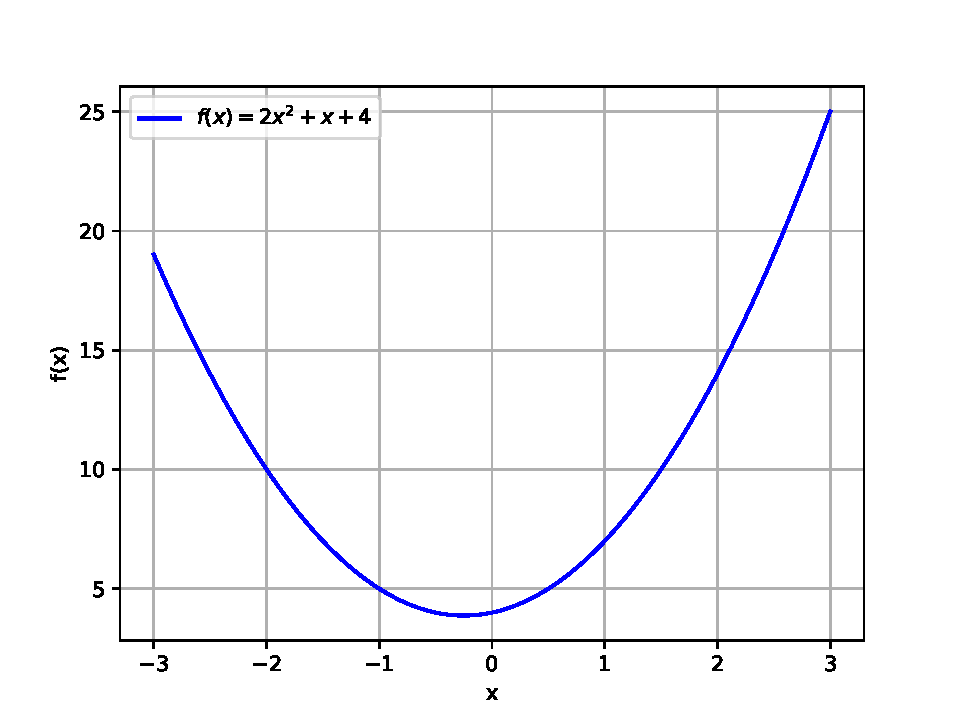
\includegraphics[width=\columnwidth]{figs/fig.pdf}
\end{figure}
\end{document}
